
\documentclass{article}
\title{Final Report: Kuwahara filter}
\author{Nguyen Dang Minh - M23.ICT.008}
\date{\today}

\usepackage{booktabs}
\usepackage{amsmath}
\usepackage{listings} % For code listings
\usepackage{xcolor}   % For defining colors
\usepackage{graphicx} 
\usepackage{float}
\usepackage{multirow}

% Define custom colors
\definecolor{codegray}{rgb}{0.95, 0.95, 0.95}
\definecolor{codepurple}{rgb}{0.58, 0, 0.82}

% Define lstlisting style
\lstdefinestyle{mystyle}{
    backgroundcolor=\color{codegray},   % Background color
    basicstyle=\footnotesize\ttfamily,  % Font style
    breaklines=true,                     % Automatically break lines
    captionpos=b,                        % Position of the caption
    commentstyle=\color{codepurple},     % Comment style
    keywordstyle=\color{blue},           % Keyword style
    language=Python,                     % Language for syntax highlighting
    numbers=left,                        % Line numbers on the left
    numbersep=5pt,                       % Space between line numbers and code
    showstringspaces=false,              % Don't show spaces in strings
    stringstyle=\color{codepurple},      % String literal style
    tabsize=4                            % Tab size
}

% Set default lstlisting style to mystyle
\lstset{style=mystyle}
\begin{document}

\maketitle
\section{Tasks:}

Apply Kuwahara filter to this image.

\begin{figure}[H]
    \centering
    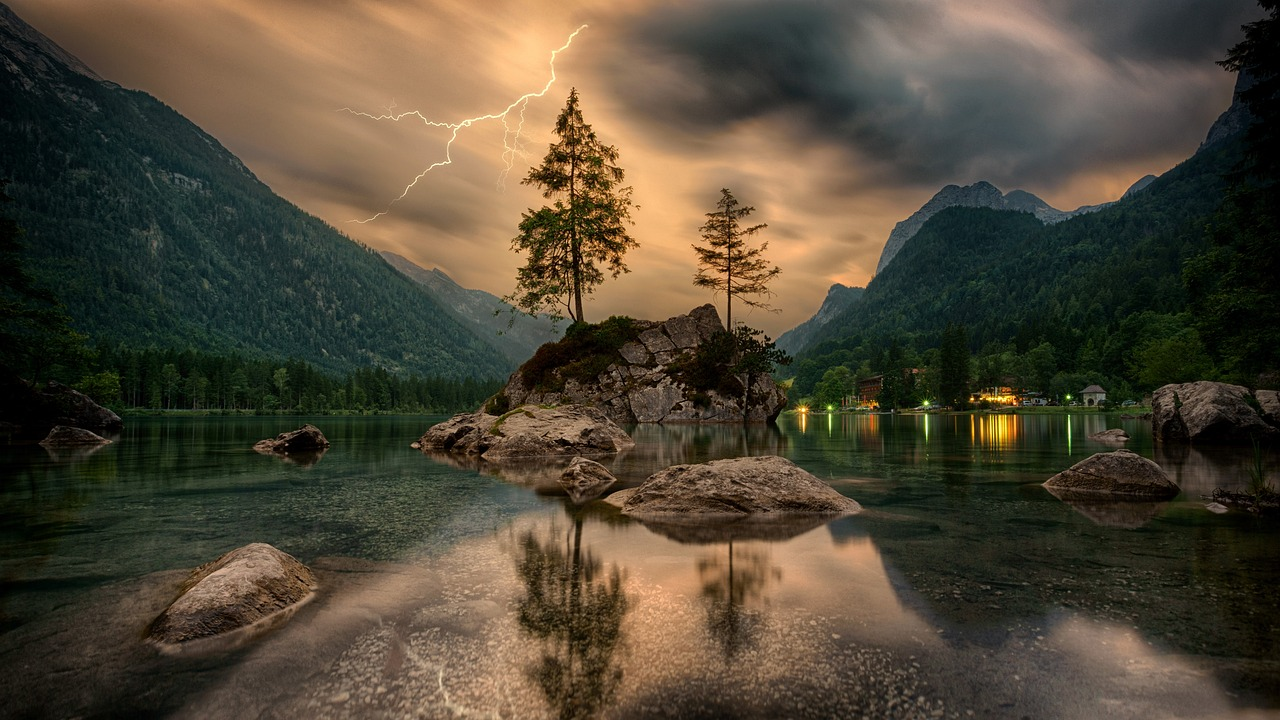
\includegraphics[width=1\linewidth]{Kuwa.jpg}
    \caption{A simple image}
\end{figure} 
Information: 
\begin{itemize}
    \item Height: 720.
    \item Width: 1280.
    \item Channel: 3.
\end{itemize}


\section{Kuwahara filter}
\subsection{Introduction}
The Kuwahara filter is a smoothing method that reduces noise while preserving edges, making it effective for image processing. 
It works by examining small regions around each pixel, calculating variations, and then selecting the region with the lowest variance to soften the pixel’s texture without blurring important details. 
It can be computationally intensive on a CPU, but the filter's simplicity and the independent calculations for each pixel make it applicable for GPU acceleration. 
The Kuwahara filter is also popular in artistic effects, where its selective smoothing creates a unique, brush-stroke look in images. 
Each Kuwahara filter have a parameter $\omega$ as the window size.

\subsection{Logic steps}
I applied Kuwahara filter in five steps:

\begin{enumerate}
    \item Pad the image to handle the edge pixel.
    \item Calculate the brightness of each pixel. 
    \item For each pixel, extract its corresponding four windows.
    \item Calculate the standard deviation of each window based on the brightness channels
    \item Assign R, G, B values for each pixel based on the mean value of the windows with the smallest standard deviation.
\end{enumerate}

\section{CPU Implementation}
\subsection{Implementation}
\subsubsection{Pad the image to handle the edge pixel}

We use the numpy.pad with mode reflect to keep the integrity of the image. 
We pad $\omega$ pixels around the input image. 

\begin{lstlisting}[language=Python]
padded_image = np.pad(image, ((w, w), (w, w), (0, 0)), mode='reflect')
\end{lstlisting}

\subsubsection{Calculate the brightness of each pixel}
Adapted from RGB to HSV
\begin{lstlisting}[language=Python]
def rgb_to_v(image):
    (H,W,_) = image.shape
    output = np.zeros((H,W), np.float32)
    for i in range(H):
        for j in range(W):
            r_v = image[i, j, 0]/255
            g_v = image[i, j, 1]/255
            b_v = image[i, j, 2]/255
            output[i, j] = max(r_v, g_v, b_v)
    return output

\end{lstlisting}

\subsubsection{Extract four windows from each pixel}
\begin{lstlisting}[language=Python]
def get_windows(image, i, j, w):
    i,j = i+w,j+w
    windows = np.zeros((4, w+1, w+1, 3), np.uint8)
    windows[0] = image[i-w:i+1, j-w:j+1, :]
    windows[1] = image[i:i+w+1, j-w:j+1, :]
    windows[2] = image[i-w:i+1, j:j+w+1, :]
    windows[3] = image[i:i+w+1, j:j+w+1, :]
    return windows
\end{lstlisting}

\subsubsection{Calculate the standard deviation of each window }
\begin{lstlisting}[language=Python]
def get_std_v(v_v,i,j,w):
    i,j = i+w,j+w
    v_list = np.zeros((4), np.float32)
    v_list[0] = np.std(v_v[i-w:i+1, j-w:j+1])
    v_list[1] = np.std(v_v[i:i+w+1, j-w:j+1])
    v_list[2] = np.std(v_v[i-w:i+1, j:j+w+1])
    v_list[3] = np.std(v_v[i:i+w+1, j:j+w+1])
    return v_list
\end{lstlisting}

\subsubsection{Assign R, G, B values for each pixel}
\begin{lstlisting}[language=Python]
def get_mean(window):
    r_v = int(np.mean(window[:,:,0]))
    g_v = int(np.mean(window[:,:,1]))
    b_v = int(np.mean(window[:,:,2]))
    return r_v,g_v,b_v
\end{lstlisting}

\subsection{Results}
\begin{figure}[H]
    \centering
    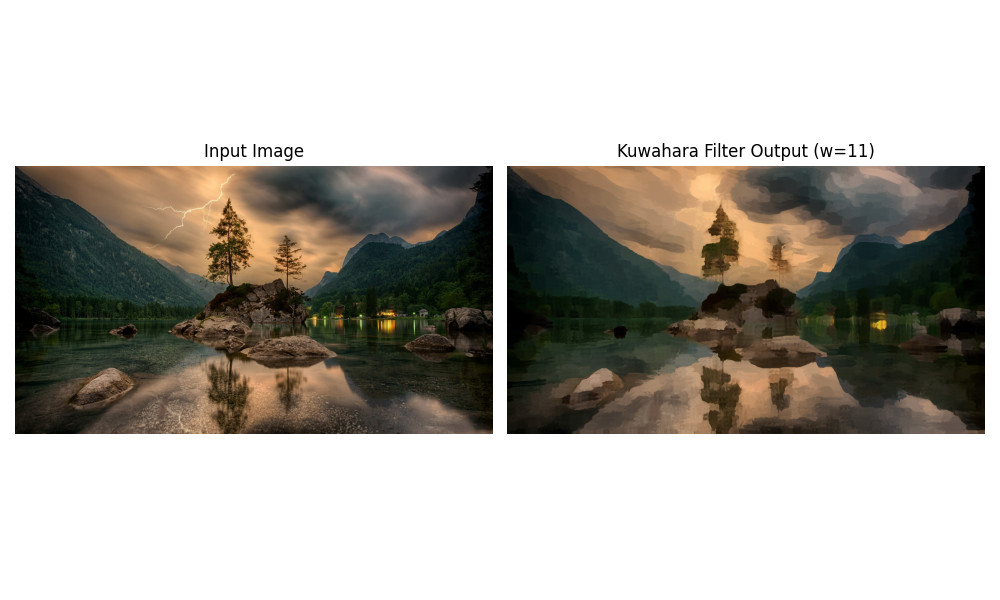
\includegraphics[width=0.9\linewidth]{Compare.png}
    \caption{Output images with different window sizes  (3, 5, 7, 9, 11)}
    \label{fig:enter-label}
\end{figure}

\section{GPU Implementation}
For the GPU implementation, I modified the order of steps slightly. 
Unlike the CPU version, which first extracts the window, then calculates the standard deviation, and selects the window with the smallest value, here I calculate the standard deviation of the four windows using only the V channel first. 
I then find the minimum to select the appropriate window. 
The initial padding step remains the same as in the CPU version.

Blocksize is (16,16)

\subsection{Without Shared Memory}
\subsubsection{Calculate the brightness of each pixel}

\begin{lstlisting}[language=Python]
@cuda.jit
def rgb_to_v_kernel(input_image, v_channel):
    x, y = cuda.grid(2)
    (H,W,_) = input_image.shape
    if y < H and x < W:
        r = input_image[y, x, 0] / 255.0
        g = input_image[y, x, 1] / 255.0
        b = input_image[y, x, 2] / 255.0
        v_channel[y, x] = max(r, g, b)
\end{lstlisting}

\subsubsection{Calculate the standard deviation of 4 windows}
\begin{lstlisting}[language=Python]
@cuda.jit(device=True)
def calculate_std(v_channel, start_x, start_y, w):
    sum_v, sum_sq_v, count = 0.0, 0.0, 0
    for i in range(0, w + 1):
        for j in range(0, w + 1):
            nx, ny = start_x + i, start_y + j
            sum_v += v_channel[ny, nx]
            count += 1
    mean = sum_v / count
    for i in range(0, w + 1):
        for j in range(0, w + 1):
            nx, ny = start_x + i, start_y + j
            v = v_channel[ny, nx]
            diff = v - mean
            sum_sq_v += diff * diff
    std = math.sqrt( sum_sq_v/ count)
    return std

\end{lstlisting}

\subsubsection{Select the smallest window }
\begin{lstlisting}[language=Python]
if w <= x < W-w and w < y < H-w:
        stds = cuda.local.array((4), numba.float32)
        stds[0] = calculate_std(v_channel, x-w, y-w, w)
        stds[1] = calculate_std(v_channel, x, y-w, w)       
        stds[2] = calculate_std(v_channel, x-w, y, w)
        stds[3] = calculate_std(v_channel, x, y, w)
        cuda.syncthreads()
        min_index = 0
        for i in range(1, 4):
            if stds[i] < stds[min_index]:
                min_index = i
        window = cuda.local.array((12, 12, 3), numba.uint8)
        start_x = x-w if min_index in [0,2] else x
        start_y = y-w if min_index in [0,1] else y
        for i in range(w + 1):
            for j in range(w + 1):
                nx = start_x + i
                ny = start_y + j
                window[i, j, 0] = input_image[ny, nx, 0]
                window[i, j, 1] = input_image[ny, nx, 1]
                window[i, j, 2] = input_image[ny, nx, 2]
\end{lstlisting}

\subsubsection{Assign R, G, B values for each pixel}
\begin{lstlisting}[language=Python]
@cuda.jit(device=True)
def calculate_mean_color(window, w):
    r_sum, g_sum, b_sum = 0, 0, 0
    count = (w + 1) ** 2
    for i in range(w + 1):
        for j in range(w + 1):
            r_sum += window[i, j, 0]
            g_sum += window[i, j, 1]
            b_sum += window[i, j, 2]
    return r_sum // count, g_sum // count, b_sum // count
\end{lstlisting}

\subsection{With Shared Memory}
To load the shared memory, we need to bring in the image data and the brightness values, along with padding of size $\omega$ for each block. 
This task is challenging due to the combined size of $\omega$ and the number of threads in each block. If $\omega$ is too large, some image data may not load correctly. 
Although loops could be used so that each pixel loads all four of its windows, this approach would ruins the benefits of parallel computing and lead to significant redundancy and wasted computation.

To simplify, each thread loads its own pixel along with the 8 pixels surrounding it within a radius of $\omega$. With this loading scheme, the filter can handle any $\omega \leq$ block size. 
The image below illustrates this loading scheme with $\omega$ set to 15 or 17 and a block size of $(16, 16)$. 
A white pixel indicates a loaded pixel, while a black pixel represents a missing pixel.


\begin{figure}[H]
    \centering
    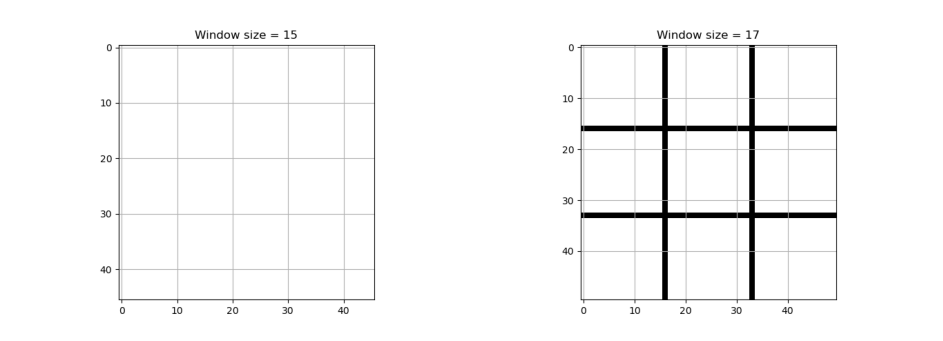
\includegraphics[width=1\linewidth]{Compare Load.png}
    \caption{Loading scheme with $\omega$ set to 15 or 17 and a block size of $(16, 16)$.}
    \label{fig:enter-label}
\end{figure}


\begin{lstlisting}[language=Python]
@cuda.jit
@cuda.jit
def load_share_mem(shared_image,shared_v,image,v,w):
    x, y = cuda.grid(2)
    x, y = x+w,y+w
    local_x, local_y = cuda.threadIdx.x, cuda.threadIdx.y 
    H, W, _ = image.shape
    if x < W-w and y< H-w:
        shared_v[local_y, local_x] = v[y, x]
        shared_v[local_y-w, local_x-w] = v[y-w, x-w]
        shared_v[local_y+w, local_x-w] = v[y+w, x-w]
        shared_v[local_y-w, local_x+w] = v[y-w, x+w]
        shared_v[local_y+w, local_x+w] = v[y+w, x+w]
        shared_v[local_y-w, local_x] = v[y-w, x]
        shared_v[local_y+w, local_x] = v[y+w, x]
        shared_v[local_y, local_x-w] = v[y, x-w]
        shared_v[local_y, local_x+w] = v[y, x+w]
        for i in range(3):
            shared_image[local_y, local_x,i] = image[y, x,i]
            shared_image[local_y-w, local_x-w,i] = image[y-w, x-w,i]
            shared_image[local_y+w, local_x-w,i] = image[y+w, x-w,i]
            shared_image[local_y-w, local_x+w,i] = image[y-w, x+w,i]
            shared_image[local_y+w, local_x+w,i] = image[y+w, x+w,i]
            shared_image[local_y-w, local_x,i] = image[y-w, x,i]
            shared_image[local_y+w, local_x,i] = image[y+w, x,i]
            shared_image[local_y, local_x-w,i] = image[y, x-w,i]
            shared_image[local_y, local_x+w,i] = image[y, x+w,i]
    cuda.syncthreads()
\end{lstlisting}

\subsection{Results}
\begin{figure}[H]
    \centering
    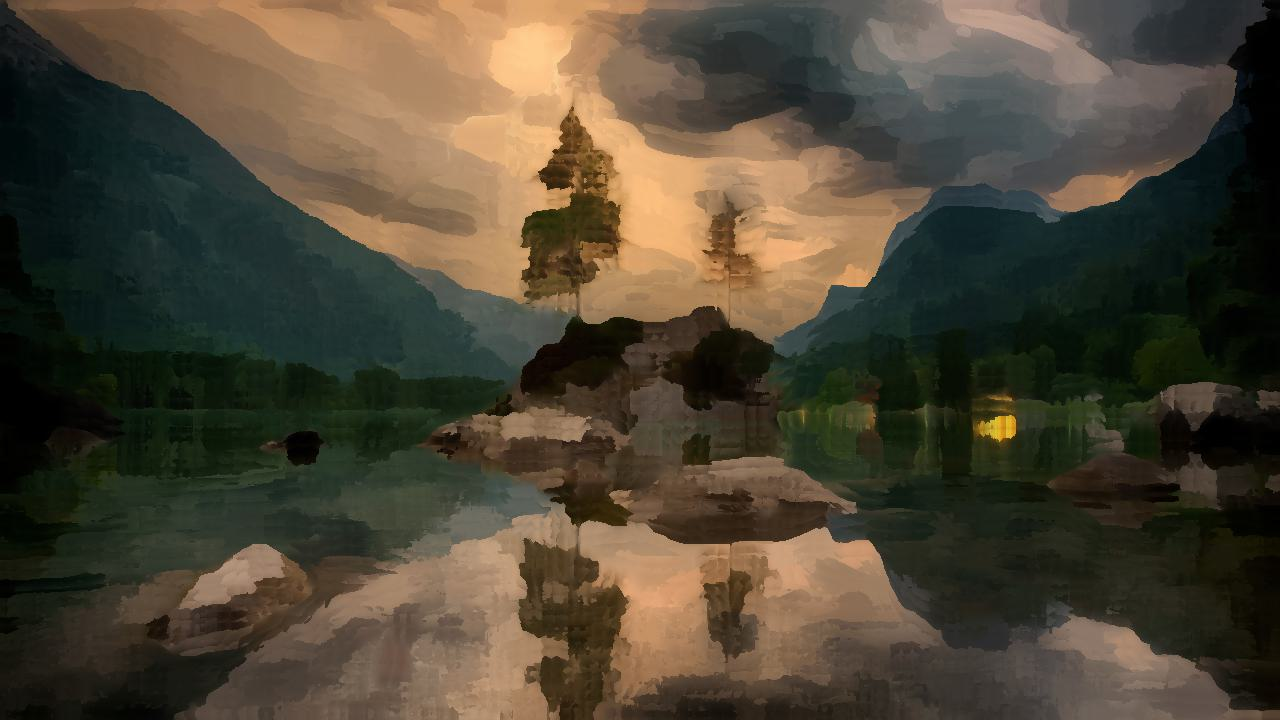
\includegraphics[width=1\linewidth]{Kuwa_GPUSM_(w=11).jpg}
    \caption{Kuwahara filter with $\omega$ = 11 using GPU}
    \label{fig:enter-label}
\end{figure}
\section{Run times comparison}

The following table presents a run time comparison between different implementations on the CPU and GPU.

\textbf{Specifications:}
\begin{itemize}
    \item \textbf{CPU}: Intel Core i7-13620H
    \item \textbf{GPU}: NVIDIA GeForce RTX 4050 Laptop GPU
\end{itemize}


\begin{table}[H]
\centering
\resizebox{\columnwidth}{!}{%
\begin{tabular}{|c|lllll|}
\hline
\multirow{2}{*}{Time (sec)} & \multicolumn{5}{c|}{Window   sizes} \\ \cline{2-6} 
            & \multicolumn{1}{c|}{3}      & \multicolumn{1}{c|}{5}      & \multicolumn{1}{c|}{7}      & \multicolumn{1}{c|}{9}      & \multicolumn{1}{c|}{11} \\ \hline
CPU         & \multicolumn{1}{l|}{60.137} & \multicolumn{1}{l|}{59.560} & \multicolumn{1}{l|}{59.531} & \multicolumn{1}{l|}{60.014} & 62.423                  \\ \hline
GPU no SM   & \multicolumn{1}{l|}{0.016}  & \multicolumn{1}{l|}{0.021}  & \multicolumn{1}{l|}{0.022}  & \multicolumn{1}{l|}{0.033}  & 0.043                   \\ \hline
GPU with SM & \multicolumn{1}{l|}{0.009}  & \multicolumn{1}{l|}{0.018}  & \multicolumn{1}{l|}{0.022}  & \multicolumn{1}{l|}{0.036}  & 0.036                   \\ \hline
\end{tabular}%
}
\caption{Runtime comparison between 3 different methods on five different window sizes}
\label{tab:my-table}
\end{table}


\begin{table}[H]
\centering

\begin{tabular}{|l|cl|}
\hline
            & \multicolumn{2}{c|}{Speed   up} \\ \hline
GPU no SM   & \multicolumn{2}{c|}{2224.350}   \\ \hline
GPU with SM & \multicolumn{2}{c|}{2494.573}   \\ \hline
\end{tabular}%

\caption{Speed up compare with CPU version}
\label{tab:my-table}
\end{table}


The results show a significant speed-up using the GPU over the CPU for all window sizes, with GPU processing times in milliseconds compared to roughly 60 seconds on the CPU.
Utilizing shared memory on the GPU further optimizes performance, especially for smaller window sizes.
Compared to the CPU, the GPU achieves a speed-up factor of 2224x, while the GPU with shared memory reaches a factor of 2495x.


\section{Conclusions & Future works}
\begin{itemize}
    \item GPU performance is much better than CPU.
    \item Shared memory optimizes performance.
\end{itemize}

\textbf{SFuture works}
\begin{itemize}
    \item Improve the shared memory loading scheme to handle bigger window size.
\end{itemize}


\end{document}